\documentclass[
    a4paper
%     ,portrait
    ,twoside
%     ,openright	% begin new chapter on right side
    ,notitlepage	% use no standard title page
%     ,10pt		% fontsize
%     ,twocolumn
%     ,french		% language
%     ,draft
  ]{article}
% 
% Load Standard Packages:
%---------------------------------------------------------------------------
\usepackage[standard-baselineskips]{cmbright}
\usepackage[ngerman]{babel}					% hyphenation
% \usepackage[frenchb]{babel}					% hyphenation	
% \usepackage[autolanguage]{numprint} 				% for french babel, must be loaded *after* babel.
% 
\usepackage[latin1]{inputenc}  					% Unix/Linux - load extended character set (ISO 8859-1)
\usepackage[T1]{fontenc}					% hyphenation of words with \"a,\"o and \"u
% \usepackage[singlespacing]{setspace} 				% 1.0x
% \usepackage[onehalfspacing]{setspace} 			% 1.5x
% \usepackage[doublespacing]{setspace} 				% 2.0x
\usepackage{csquotes}						% added by brugr9: used for babel
\usepackage{textcomp}						% additional symbols
% \usepackage{ae}						% better resolution of Type1-Fonts
\usepackage{fancyhdr}						% simple manipulation of header and footer
\usepackage{etoolbox}						% color manipulation of header and footer
\usepackage{graphicx}                      			% integration of images
\usepackage{float}						% floating objects
\usepackage{caption}						% for captions of figures and tables
\usepackage{booktabs}						% package for nicer tables
\usepackage{tocvsec2}						% provides means of controlling the sectional numbering
%---------------------------------------------------------------------------
% 
% Package to facilitate placement of boxes at absolute positions
%---------------------------------------------------------------------------
\usepackage[absolute]{textpos}
\setlength{\TPHorizModule}{1mm}
\setlength{\TPVertModule}{1mm}
%---------------------------------------------------------------------------
% 
% Definition of Colors
%---------------------------------------------------------------------------
\RequirePackage{color} 						% Color (not xcolor!)
\definecolor{linkblue}{rgb}{0,0,0.8} 				% Standard
\definecolor{darkblue}{rgb}{0,0.08,0.45} 			% Dark blue
% 
\definecolor{red}{rgb}{0.97,0,0}
% 
% \definecolor{linkcolor}{rgb}{0,0,0.8}     			% Blue for the web- and cd-version!
\definecolor{linkcolor}{rgb}{0,0,0}        			% Black for the print-version!
%---------------------------------------------------------------------------
% 
% Hyperref Package (Create links in a pdf)
% PDF-property title, author and subject
%---------------------------------------------------------------------------
\usepackage[
	pdftex,bookmarks,plainpages=false,pdfpagelabels,
% 	,british
% 	,ngerman
% 	,frenchb
	backref 	= {false},				% No index backreference
	colorlinks 	= {true}, 				% Color links in a PDF
	hypertexnames 	= {true}, 				% no failures "same page(i)"
	bookmarksopen 	= {true}, 				% opens the bar on the left side
	bookmarksopenlevel = {1}, 				% depth of opened bookmarks
% 	TODO PDF-properties
	pdftitle 	= {H34RTB34T}, 				% PDF-property title
	pdfauthor 	= {Roland\ Bruggmann}, 			% PDF-property author
	pdfsubject 	= {Biomedical\ Instrumentation\ and\ Electrical\ Engineering}, 	% PDF-property subject
% 	
	linkcolor 	= {linkcolor}, 				% Color of Links
	citecolor 	= {linkcolor}, 				% Color of Cite-Links
	urlcolor 	= {linkcolor}, 				% Color of URLs
]{hyperref}
%---------------------------------------------------------------------------
% 
% Set up page dimension
%---------------------------------------------------------------------------
\usepackage{lastpage}
\usepackage{multicol}
\usepackage{geometry}
\geometry{
	a4paper,
	left=28mm,
	right=15mm,
	top=30mm,
	headheight=20mm,
	headsep=10mm,
	textheight=242mm,
	footskip=15mm
}
%---------------------------------------------------------------------------
% 
% Divers by brugr9
%---------------------------------------------------------------------------
\usepackage{units}
\usepackage{
   amssymb
  ,amsmath 		% AMS mathematics
%   ,amsthm 		% for theorem
}
% \usepackage{footmisc}
\usepackage{lmodern}
% \usepackage{lipsum} 				% to generate filler text
%---------------------------------------------------------------------------
% 
% Glossary
%---------------------------------------------------------------------------
% \usepackage[
%   nonumberlist
%   ,nopostdot
%   ,acronym
%   ]{glossaries}
% \makeglossaries
% \loadglsentries{./datenbanken/glossary}
%---------------------------------------------------------------------------
% 
% Bibliography
%---------------------------------------------------------------------------
\usepackage[
      style=alphabetic
%       style=numeric
      ,defernumbers=true
      ,backend=biber
%       ,isbn=false
    ]{biblatex}
\addbibresource{./datenbanken/bibliography.bib}
%---------------------------------------------------------------------------
% 
\newcommand{\matlab}{{\small\textsc{Matlab}\textsuperscript{{\tiny\textregistered}} }}
\newcommand{\mathworks}{{\small\textsc{Mathworks}\textsuperscript{{\tiny\textregistered}} }}
% 
\newcommand{\arcustan}[2]{\arctan \left(\frac{#1}{#2}\right)}
% 
% Start document
%---------------------------------------------------------------------------
\begin{document}
\providecommand{\Modul}{Biomedical Instrumentation and \\Introduction to Electronical Engineering}
\providecommand{\Titel}{H34ARTB34T}
\providecommand{\Untertitel}{Do-it-yourself Electrocardiogram}
\providecommand{\ArtDerArbeit}{Semesterwork}
\providecommand{\Autor}{Roland Bruggmann}
\providecommand{\Institution}{Faculty of Medicine, University of Bern.}
\providecommand{\Ort}{Bern}
% \providecommand{\Versionsdatum}{Dezember 2017}
\providecommand{\Versionsdatum}{\today}
\providecommand{\Version}{Version 0.1}
% %   
% 
% % Glossar
% 
% \newglossaryentry{gEnterpriseArchitectureFramework}
% {
%   name={Enterprise Architecture Framework},
%   description={Ein Enterprise Architecture Framework (EAF, dt. Unternehmensarchitekturrahmenwerk) ist ein Mittel f\"ur das IT-Management zur Planung, Realisierung und Weiterf\"uhrung von Unternehmensarchitekturen in der Informationstechnologie.}
% }
% 
% 
% 
% % Acronyms
% 
% ---------------------------------------------------------
% 
% \newacronym{SWEEP}{SWEEP}{Sensor \dots}
% \glsaddall
%---------------------------------------------------------------------------
% 
% Set up header and footer
%---------------------------------------------------------------------------
\makeatletter
% \patchcmd{\@fancyhead}{\rlap}{\color{black}\rlap}{}{} 	% new color of header
\makeatother
% 
\fancyhf{} 							% clean all fields
\fancypagestyle{plain}{ 					% new definition of plain style
	\fancyhead[R]{\footnotesize \Modul} 			% header right part
	\fancyhead[L]{\footnotesize 
	    
\includegraphics[scale=0.4]{./graphics/unibe-logo-120px.png} \Institution}		% header left part
% 	\fancyfoot[R]{\footnotesize 
% 	    Page \thepage\hspace{2pt}
% 	    \hypersetup{linkcolor=black}(\pageref{LastPage})} % footer right part
	\fancyfoot[R]{\footnotesize 
	    Seite \thepage\hspace{2pt}
	    \hypersetup{linkcolor=black}(\pageref{LastPage})} % footer right part
% 	    
	\fancyfoot[L]{\footnotesize 
	    {\Titel, \Version\ }| \Autor}	% footer left part
}
% 
% \renewcommand{\chaptermark}[1]{\markboth{\thechapter.  #1}{}}
\renewcommand{\headrulewidth}{0pt}				% header stripline
\renewcommand{\footrulewidth}{0pt} 				% bottom stripline
% 
\pagestyle{plain}
\pagenumbering{arabic}
\setcounter{page}{1}
%---------------------------------------------------------------------------
% 
% Titelei
%---------------------------------------------------------------------------
% 
% \maketitle 
% 
\setlength{\unitlength}{1mm}
\begin{flushleft}
    \begin{picture}(167,1.0)
	    \put(0,0){\color{black}\rule{167mm}{1.5mm}}
    \end{picture}
    \begin{tabbing}
	    xxxxx\=xxxxxxxxxxxxxxxxxxxxxxxxxxxxxxxxxxxxxxxxxxxxxxxxxxxxxxxxx \kill
	    \> \color{white}\textbf{\Untertitel} \\
	    \> \\
	    \> \color{white}\LARGE\textbf{\Titel} \\
    \end{tabbing}
    \begin{picture}(167,1.0)
	    \put(0,0){\color{black}\rule{167mm}{1.5mm}}
    \end{picture}
\end{flushleft}
% 
\begin{textblock}{20}[0,0](28,60) % f\"ur 12pt: l 28, t 66
      \begin{picture}(167,1.0)
	    \put(0,0){\color{red}\rule{167mm}{28mm}} % f\"ur 12pt: 167mm/33mm
      \end{picture}
\end{textblock}
%---------------------------------------------------------------------------

\begin{multicols*}{2} % like twocolumn
% 
% Portrait
%---------------------------------------------------------------------------
% 
\begin{flushleft}
  \footnotesize
  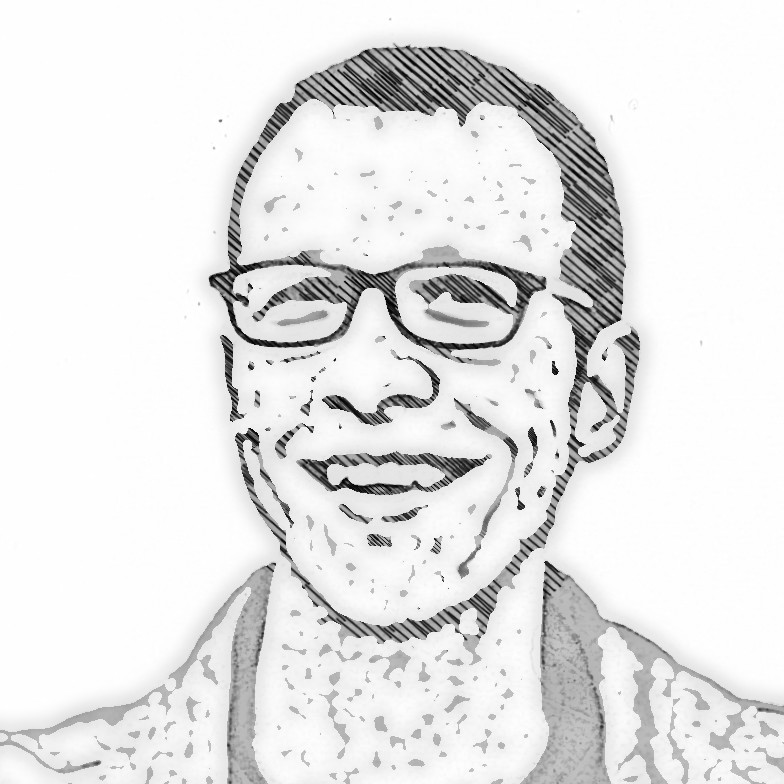
\includegraphics[
      scale=0.08
      ,keepaspectratio=true
      ,clip=true
      ,trim=0pt 0pt 0pt 0pt
      ]{./graphics/portrait-2002-cut-pencil-2.jpg}
      % trim: l, b, r, t
  % 1317x875 pixel, 72dpi, 46.46x30.86 cm, bb=0 0 1317 875
  \vspace*{-3mm}
  \\\rule{150pt}{2.0pt}
  \vspace*{1mm}
  \\\textbf{\Autor}
  \scriptsize
% 
  \vspace*{1pt}\\Student MSc in Biomedical Engineering BME
  \vspace*{-3pt}\\\href{mailto:roland.bruggmann@students.unibe.ch}{\nolinkurl{roland.bruggmann@students.unibe.ch}}
  \normalsize
\end{flushleft}
\vspace*{-8pt}
%---------------------------------------------------------------------------

% \fontsize{12bp}{14bp}\selectfont
\smallskip
\begin{flushleft}
  \footnotesize
  \textbf{\Ort, \Versionsdatum}
  \normalsize
\end{flushleft}
\vspace*{-8pt}
\smallskip

%---------------------------------------------------------------------------
% 
% Content
% \psq
% \psqq
%---------------------------------------------------------------------------
% \section*{Problemstellung} 
Eine digitale Authentifikation erfolgt heutzutage meist \"uber ein Benutzerkonto, bestehend aus Benutzername und Passwort. Mit dem Eintippen eines Benutzernamens wird eine Identit\"at propagiert, \"uber das Passwort findet die Verifikation statt. St\"arkere Sicherheit bieten jedoch Methoden der Biometrie. Eine Person liefert eine Probe zur Identifikation, es erfolgt ein Vergleich der Probe mit den Referenzdaten im System. 

Ein wichtiges physiologisches Attribut einer nat\"urlichen Person ist ihr Fingerabdruck. Dieser kann als messbarer Identifikator dienen. Dazu muss der Abdruck eine Analyse durchlaufen, damit charakteristische Merkmale im Rillenbild extrahiert und verglichen werden k\"onnen. 

Mit dieser Semesterarbeit wollen wir Algorithmen von bekannten Methoden der Biometrie zur Merkmalsextraktion am Fingerabdruck implementieren. Als Softwarel\"osung im Sinne eines Prototypen wird ein Skript in \matlab programmiert. 
    
\section*{Method}
(see fig.~\ref{fig:platzhalter}).
\begin{figure}[H]
  \centering
      \fbox{
      
\includegraphics[
% 	width=107pt
	scale=0.35
	,keepaspectratio=true
	,clip=true,trim=90pt 65pt 95pt 30pt % trim: l, b, r, t
	]{./images/platzhalter.jpg}
	}
  \caption{platzhalter}
  \label{fig:platzhalter}
\end{figure}

\section*{Results}

\section*{Discusion}

\section*{Conclusion}

\scriptsize{$\square$}\normalsize

% \the\baselineskip 	% zeilenabstand anzeigen
% 
%---------------------------------------------------------------------------
% References
%---------------------------------------------------------------------------
\bigskip
\begingroup
\let\clearpage\relax
% \renewcommand{\refname}{\normalsize\textbf{Literatur}}
% \renewcommand*{\bibfont}{\scriptsize}
% 
% Books
% \nocite{Gil15} 	% Matlab
% \nocite{Len13} 	% Matlab
\nocite{GWE04} 		% Matlab, Image Processing
\nocite{Mal09} 		% Biometry
% 
% Papers
\nocite{BG02} 		% Biometry
% \nocite{JRP04} 	% Biometry
% \nocite{Cap07} 	% Biometry, FVC2006
% 
% Data
\nocite{FVC04} 	% Biometry
% 
% Software
% \nocite{IPT} 		% Matlab
% \nocite{DIPUM} 	% Matlab, Image Processing
% 
% Teaching material
% \nocite{Hud15} 	% Image Processing
% \nocite{Mul15} 	% Biometry
% \nocite{Sta15} 	% Matlab

\printbibliography
\endgroup
%---------------------------------------------------------------------------
% 
\end{multicols*}
% 
\end{document}